% https://nymity.ch/tikz/

\documentclass[hyperref={pdfpagelabels=true},table,dvipsnames,14pt,aspectratio=169]{beamer}
\usetheme{Boadilla}
\setbeamertemplate{navigation symbols}{}

\usepackage{amsthm, amsfonts, amssymb, amsmath, graphicx}
\usepackage{amsmath}
\usepackage{amsfonts, txfonts}
\usepackage{wasysym}
\usepackage{xcolor}
\usepackage{caption}
\usepackage{comment}

\usepackage{graphicx}
\graphicspath{ {images/} }

\usepackage{tikz}
\usepackage{tikzpeople}
\usepackage{pgfplots}
\pgfplotsset{compat=1.15}
\usetikzlibrary{arrows}

% Method to add an item that will appear in every slide
%\addtobeamertemplate{footline}{%
%
%  \tikz[remember picture, overlay] \fill[blue] (current page.south east)
%    rectangle ++(1cm,2cm);
%
%}{}

\pgfdeclareimage[height=5ex]{crysplogo}{crysplogo}
\pgfdeclareimage[height=5ex]{cscslogo}{cscslogo}
\pgfdeclareimage[height=5ex]{torlogo}{torlogo}
\pgfdeclareimage[height=1.5ex]{clikey}{key}
\pgfdeclareimage[height=1.5ex]{srvkey}{key-green}
\pgfdeclareimage[height=1.5ex]{clivrfkey}{key-blue}
\pgfdeclareimage[height=1.5ex]{srvvrfkey}{key-red}
\pgfdeclareimage[height=1cm]{server}{server}

\titlegraphic{
%\raisebox{1ex}{
%\pgfuseimage{crysplogo}~~~
\pgfuseimage{cscslogo}~~~
\pgfuseimage{torlogo}
%}
}

\definecolor{AlertRed}{rgb}{1.0,0.125,0.25}
\setbeamercolor{alerted text}{fg=AlertRed}
%\setbeamerfont{alerted text}{shape=\bfseries,size=\huge}
\definecolor{auth}{RGB}{138,23,94}

\newcommand\shortdoc{
\begin{tikzpicture}[scale=.25] \draw[-,draw=black,fill=gray] (0,0) -- (2,0) -- (2,-2) -- (-1,-2) -- (-1,-1) -- cycle; \end{tikzpicture}}
\newcommand\shortdocused{
\begin{tikzpicture}[scale=.25]
\draw[-,draw=black,fill=green] (0,0) -- (2,0) -- (2,-2) -- (-1,-2) -- (-1,-1) -- cycle; \end{tikzpicture}}

\newcommand\medconsensus{
\begin{tikzpicture}[scale=.25] \draw[-,draw=black,fill=gray] (0,0) -- (2,0) -- (2,-6) -- (-1,-6) -- (-1,-1) -- cycle; \node[shape=star,star points=9,fill=auth,inner sep=0pt,star point ratio=.5,minimum size=2mm,anchor=south east] at (1.8,-5.8) {} ; \end{tikzpicture}}
\newcommand\longconsensus{
\begin{tikzpicture}[scale=.25] \draw[-,draw=black,fill=gray] (0,0) -- (2,0) -- (2,-13) -- (-1,-13) -- (-1,-1) -- cycle; \node[shape=star,star points=9,fill=auth,inner sep=0pt,star point ratio=.5,minimum size=2mm,anchor=south east] at (1.8,-12.8) {} ; \end{tikzpicture}}
\newcommand\netdocunsigned{
\begin{tikzpicture}[scale=.25] \draw[-,draw=black,fill=ProcessBlue] (0,0) -- (2,0) -- (2,-2) -- (-1,-2) -- (-1,-1) -- cycle; \end{tikzpicture}}
\newcommand\netdoc{
\begin{tikzpicture}[scale=.25] \draw[-,draw=black,fill=ProcessBlue] (0,0) -- (2,0) -- (2,-2) -- (-1,-2) -- (-1,-1) -- cycle; \node[shape=star,star points=9,fill=auth,inner sep=0pt,star point ratio=.5,minimum size=2mm,anchor=south east] at (1.8,-1.8) {} ; \end{tikzpicture}}
\newcommand\snipdoc{
\begin{tikzpicture}[scale=.25] \draw[-,draw=black,fill=LimeGreen] (0,0) -- (2,0) -- (2,-2) -- (-1,-2) -- (-1,-1) -- cycle; \node[shape=star,star points=9,fill=auth,inner sep=0pt,star point ratio=.5,minimum size=2mm,anchor=south east] at (1.8,-1.8) {} ; \end{tikzpicture}}
\newcommand\docendive{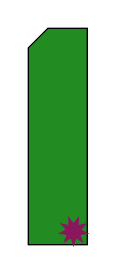
\begin{tikzpicture}[scale=.25] \draw[-,draw=black,fill=ForestGreen] (0,0) -- (2,0) -- (2,-11) -- (-1,-11) -- (-1,-1) -- cycle; \node[shape=star,star points=9,fill=auth,inner sep=0pt,star point ratio=.5,minimum size=2mm,anchor=south east] at (1.8,-10.8) {} ; \end{tikzpicture}}
\newcommand\snipdocunsigned{
\begin{tikzpicture}[scale=.25] \draw[-,draw=black,fill=LimeGreen] (0,0) -- (2,0) -- (2,-2) -- (-1,-2) -- (-1,-1) -- cycle; \end{tikzpicture}}


\pgfdeclarelayer{background}
\pgfdeclarelayer{backbackground}
\pgfdeclarelayer{foreground}
\pgfsetlayers{backbackground,background,main,foreground}   %% some additional layers for demo

\usetikzlibrary{shapes,decorations.shapes}
\tikzset{>=latex}


\title[Walking Onions]{Walking Onions: Scaling Anonymity Networks while Protecting Users}
\author{\textbf{Chelsea Komlo}, Nick Mathewson, Ian Goldberg}
%\institute{\small{Presented at USENIX Security}}
\date{Presented at USENIX Security \\ 13 August, 2020}

\begin{document}
\setbeamertemplate{itemize items}[triangle]

\begin{frame}
        \thispagestyle{empty}
        \maketitle
\end{frame}


\begin{frame}
\frametitle{Motivation}
  \begin{itemize}
    \item<1-> \textbf{Enable Scalability.} Remove the requirement that every
      client maintains up-to-date information about every relay, a current
      requirement for security.
    \item<1>[]~
    \item<2> \textbf{Maintain User Safety.} Maintain the existing security model of Tor.
  \end{itemize}
\end{frame}

\begin{frame}
\frametitle{What Contributions Does Walking Onions Make?}
  \begin{itemize}
    \item<1-> \textbf{Improved Scalability.} Constant-size bandwidth overhead for
      clients even as new relays are added to the network.
    \item<1->[]~
    \item<2-> \textbf{Maintains Tor's Existing Security Model.} One variant has no change,
      the other a slight loss of forward secrecy.
    \item<2->[]~
    \item<3-> \textbf{Immediate Performance Improvements.} Demonstrates
      improvements at networks the size of Tor today.
  \end{itemize}
\end{frame}

\begin{frame}
  \centering
  \huge
  Current Tor
\end{frame}

\begin{frame}
\frametitle{What is Tor's Existing Security Model?}

  \begin{itemize}
    \item<1-> \textbf{Epistemic Attacks}: Users with different views of the
      network can be distinguished by their relay selection.
    \item<1->[]~
    \item<2-> \textbf{Route-Capture Attacks}: When an adversary can influence
      users' relay selection.
  \end{itemize}

\end{frame}

\begin{frame}
\frametitle{Current Tor Path Selection and Circuit Extension}
\footnotesize
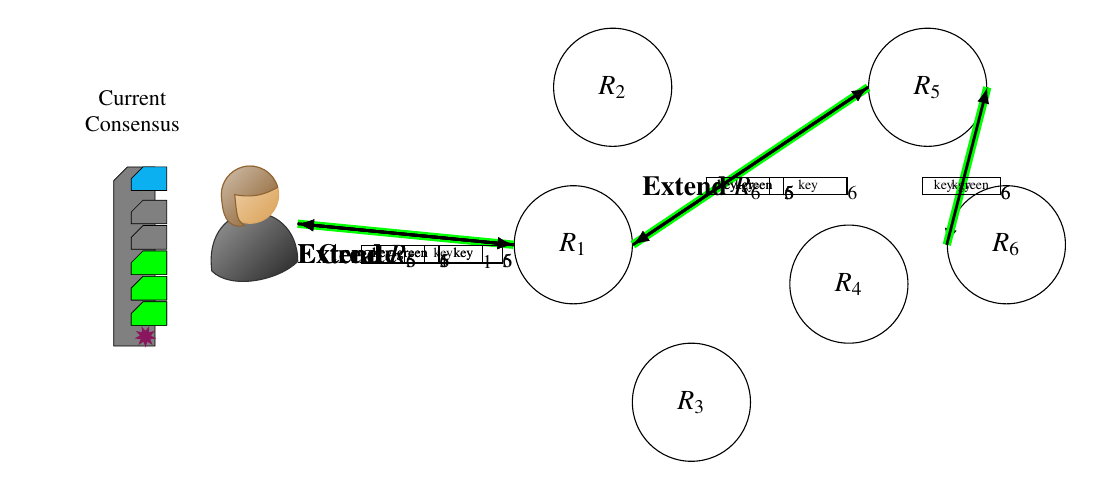
\begin{tikzpicture}
  \node[person,shirt=black,female,minimum size=1.1cm] (user1) at (-5,-1) {};

  \begin{pgfonlayer}{backbackground}
    \node [anchor=north,inner sep=0pt] (cons) at ($(user1.north west)+(-1,0)$)
      {\scalebox{.7} {  \longconsensus} };
    \node [font=\footnotesize,text centered,text width=.2\textwidth] (constitle) at
    ($(cons.north)+(0,.7)$) {Current\\Consensus};
    \node [anchor=north,inner sep=0pt] (netdoc) at ($(cons.north east)+(-.1,0)$)
    {\scalebox{0.6} {\netdocunsigned }};
    \node [anchor=north,inner sep=0pt] (d0) at ($(netdoc.south)+(0,-.1)$)
    {\scalebox{0.6} {\shortdoc}};
    \node [anchor=north,inner sep=0pt] (d1) at (d0.south)
    {\scalebox{0.6} {\shortdoc}};
    \node [anchor=north,inner sep=0pt] (d2) at (d1.south) {\scalebox{0.6}
    {\shortdoc}};
    \node [anchor=north,inner sep=0pt] (d3) at (d2.south) {\scalebox{0.6}
    {\shortdoc}};
    \node [anchor=north,inner sep=0pt] (d4) at (d3.south) {\scalebox{0.6}{\shortdoc}};
  \end{pgfonlayer}

  \begin{pgfonlayer}{background}
    \node[circle,draw,minimum size=1.5cm] (R1) at
    ($(user1.north east)+(3.5,-1)$) {$R_1$};
    \node[circle,draw,minimum size=1.5cm] (R2) at
    ($(user1.north east)+(4,1)$) {$R_2$};
    \node[circle,draw,minimum size=1.5cm] (R3) at
    ($(user1.north east)+(5,-3)$) {$R_3$};
    \node[circle,draw,minimum size=1.5cm] (R4) at
    ($(user1.north east)+(7,-1.5)$)  {$R_4$};
    \node[circle,draw,minimum size=1.5cm] (R5) at
    ($(user1.north east)+(8,1)$)  {$R_5$};
    \node[circle,draw,minimum size=1.5cm] (R6) at
    ($(user1.north east)+(9,-1)$)  {$R_6$};
  \end{pgfonlayer}

    \draw<1>[line width=1pt,->] (user1.east) -- (R1.west) node [below, midway]
    {\textbf{Create} $\pgfuseimage{clikey}_1$};
    \node<1->[anchor=north,inner sep=0pt] (d4) at (d3.south)
     {\scalebox{0.6}{\shortdocused}};

    \draw<2->[draw=green, line width=3pt,-] (user1.east) -- (R1.west) node
    [below, midway] {};
    \draw<2>[line width=1pt,->] (R1.west) -- (user1.east) node [below, midway]
    {$\pgfuseimage{srvkey}_1$};

    \draw<3>[line width=1pt,->] (user1.east) -- (R1.west) node [below, midway]
    {\textbf{Extend} $R_5$ $\pgfuseimage{clikey}_5$};
    \node<3->[anchor=north,inner sep=0pt] (d3) at (d2.south)
    {\scalebox{0.6}{\shortdocused}};

    \draw<4>[line width=1pt,->] (R1.east) -- (R5.west) node [below, midway]
    {$\pgfuseimage{clikey}_5$};


    \draw<5->[draw=green, line width=3pt,-] (R1.east) -- (R5.west) node {};
    \draw<5>[line width=1pt,->] (R5.west) -- (R1.east) node [below, midway]
    {$\pgfuseimage{srvkey}_5$};

    \draw<6>[line width=1pt,->] (R1.west) -- (user1.east) node [below, midway]
    {$\pgfuseimage{srvkey}_5$ };

    \draw<7>[line width=1pt,->] (user1.east) -- (R1.west) node [below, midway]
    {\textbf{Extend} $R_6$ $\pgfuseimage{clikey}_6$};
    \node<7->[anchor=north,inner sep=0pt] (d2) at (d1.south)
    {\scalebox{0.6}{\shortdocused}};

    \draw<8>[line width=1pt,->] (R1.east) -- (R5.west) node [below, midway]
    {\textbf{Extend} $R_6$ $\pgfuseimage{clikey}_6$};

    \draw<9>[line width=1pt,->] (R5.east) -- (R6.west) node [below, midway]
    {$\pgfuseimage{clikey}_6$};

    \draw<10->[draw=green, line width=3pt,-] (R5.east) -- (R6.west) node {};
    \draw<10>[line width=1pt,->] (R6.west) -- (R5.east) node [below, midway]
    {$\pgfuseimage{srvkey}_6$};

    \draw<11>[line width=1pt,->] (R5.west) -- (R1.east) node [below, midway]
    {$\pgfuseimage{srvkey}_6$};

    \draw<12>[line width=1pt,->] (R1.west) -- (user1.east) node [below, midway]
    {$\pgfuseimage{srvkey}_6$};

\end{tikzpicture}
\end{frame}

\begin{frame}
\frametitle{Tor Security Model: Security over Scalability}
  \begin{itemize}
    \item<1-> \textbf{Globally Consistent View.} Consensus size grows quadratically
      relative to the number of relays, which all clients must maintain!
    \item<1->[]~
    \item<2-> \textbf{Goal:}
      \begin{itemize}
        \item<3-> Same protections against eptistemic and route
      capture attacks, but
        \item<3->[]~
        \item<4->  \emph{Without} requiring clients to hold a globally
          consistent network view.
      \end{itemize}
  \end{itemize}
\end{frame}

\begin{frame}{What improvements does Walking Onions make?}
  \begin{itemize}
    \item<1-> How to represent relay information to enable oblivious
      selection and individual verification?
    \item<2->[]~
    \item<2-> How to build paths using oblivious relay selection?
    \item<2->[]~
    \item<3-> How to perform more efficient circuit construction?
  \end{itemize}
\end{frame}

\begin{frame}{What improvements does Walking Onions make?}
  \begin{itemize}
    \item<1-> \textbf{How to represent relay information to enable oblivious
      selection and individual verification?}
    \item<1->[]~
    \item<1->[]~
    \item<1->[]~
    \item<1->[]~
  \end{itemize}
\end{frame}


\begin{frame}
  \frametitle{New Data Structure: Seperable Network Index Proof (SNIP)}
\centerline{%
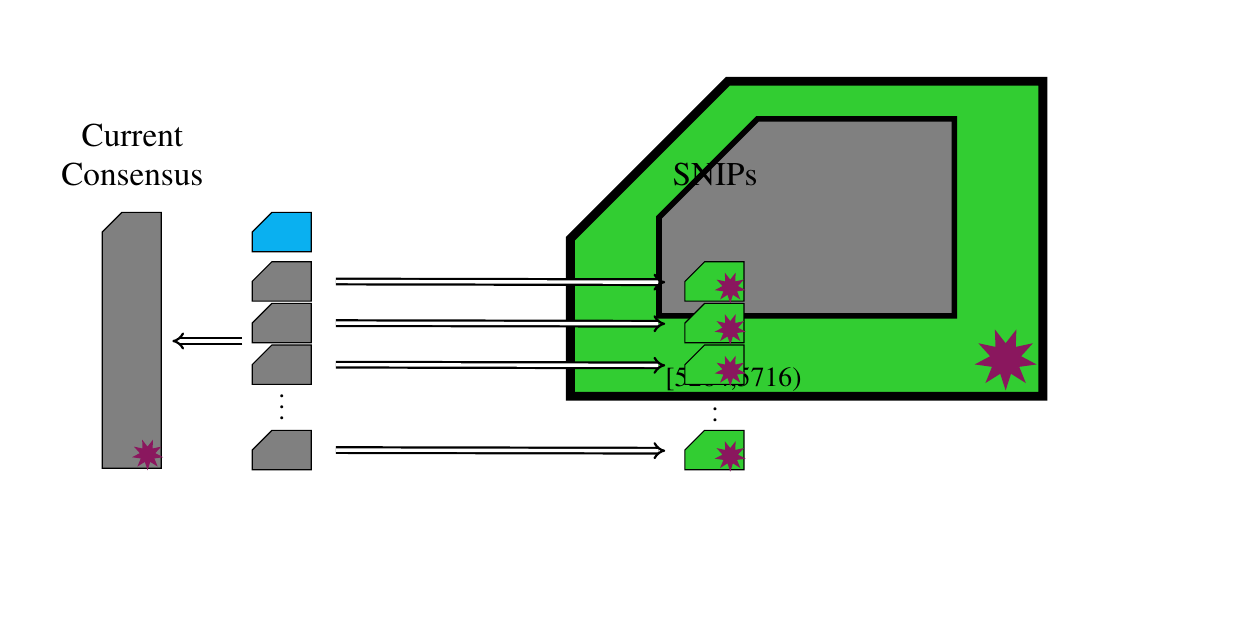
\begin{tikzpicture}
\node at (-7,-3.5) {~};
\node at (7,3.5) {~};
\node [font=\large,text centered,text width=.2\textwidth] (constitle) at (-6.5,2) {Current\\Consensus};
\node [anchor=north,inner sep=0pt] (cons) at ($(constitle.south) + (0,-.2)$) {\longconsensus};
\node [anchor=north,inner sep=0pt] (netdoc) at ($(cons.north east)+(1.5,0)$) {\netdocunsigned};
\node [anchor=north,inner sep=0pt] (d1) at ($(netdoc.south)+(0,-.1)$) {\shortdoc};
\node [anchor=north,inner sep=0pt] (d2) at (d1.south) {\shortdoc};
\node [anchor=north,inner sep=0pt] (d3) at (d2.south) {\shortdoc};
\node [anchor=south,inner sep=0pt] (d4) at ($(cons.south west)!(d2.south)!(cons.south east)$) {\shortdoc};
\node [anchor=north,inner sep=0pt] at ($(d3.south)+(0,.1)$) {$\mathbf{\vdots}$};
\draw [line width=2pt,double,thick,double equal sign distance,-implies] ($($(netdoc.north west)!(cons.east)!(netdoc.south west)$)!.1!(cons.east)$) -- ($($(netdoc.north west)!(cons.east)!(netdoc.south west)$)!.9!(cons.east)$);
\node<2> [anchor=north west,inner sep=0pt] (snip) at (-1,3) {\scalebox{8}{\snipdocunsigned}};
\node<2> [anchor=north,inner sep=0pt] (snipdesc) at ($(snip.north)+(0,-.5)$) {\scalebox{5}{\shortdoc}};
\node<2> [anchor=south west] at ($(snip.south west)!(snipdesc.south west)!(snip.south east)$) {[5284,5716)};
\node<2> [shape=star,star points=9,fill=auth,inner sep=0pt,star point ratio=.5,minimum size=4mm,anchor=south east] at ($(snip.south east)+(-.3,.3)$) {} ;
\node<3-> [font=\large,anchor=south] (sniptitle) at
  ($(constitle.south west)!(.9,3)!(constitle.south east)$) {SNIPs};
\node<3-> [anchor=north,inner sep=0pt] (snip1) at ($(sniptitle.north)!(d1.north)!(sniptitle.south)$) {\snipdoc};
\node<3-> [anchor=north,inner sep=0pt] (snip2) at ($(sniptitle.north)!(d2.north)!(sniptitle.south)$) {\snipdoc};
\node<3-> [anchor=north,inner sep=0pt] (snip3) at ($(sniptitle.north)!(d3.north)!(sniptitle.south)$) {\snipdoc};
\node<3-> [anchor=north,inner sep=0pt] at ($(snip3.south)+(0,.1)$) {$\mathbf{\vdots}$};
\node<3-> [anchor=north,inner sep=0pt] (snip4) at ($(sniptitle.north)!(d4.north)!(sniptitle.south)$) {\snipdoc};
\draw<3-> [line width=2pt,double,thick,double equal sign distance,-implies] ($(d1.east)!.3cm!(snip1.west)$) -- ($(d1.east)!.95!(snip1.west)$);
\draw<3-> [line width=2pt,double,thick,double equal sign distance,-implies] ($(d2.east)!.3cm!(snip2.west)$) -- ($(d2.east)!.95!(snip2.west)$);
\draw<3-> [line width=2pt,double,thick,double equal sign distance,-implies] ($(d3.east)!.3cm!(snip3.west)$) -- ($(d3.east)!.95!(snip3.west)$);
\draw<3-> [line width=2pt,double,thick,double equal sign distance,-implies] ($(d4.east)!.3cm!(snip4.west)$) -- ($(d4.east)!.95!(snip4.west)$);
\end{tikzpicture}
}
\end{frame}

\begin{frame}
\frametitle{ENDIVE: Efficient Network Directory with Independently Verifiable
  Entries }
\centerline{%
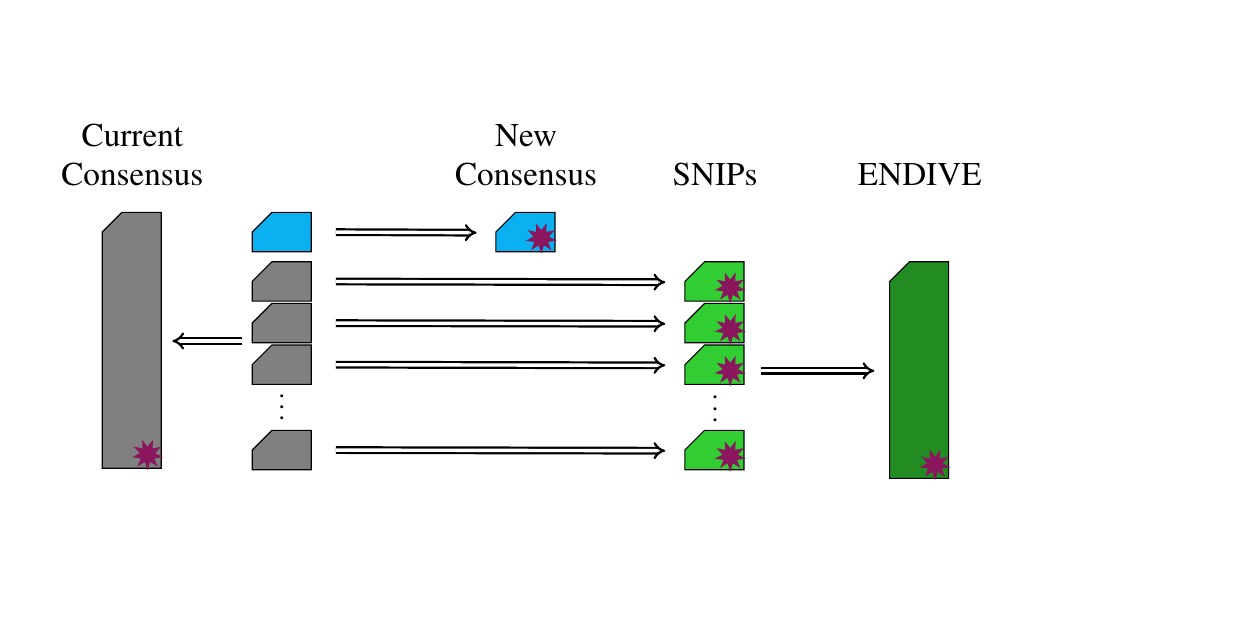
\begin{tikzpicture}
\node at (-7,-3.5) {~};
\node at (7,3.5) {~};
\node [font=\large,text centered,text width=.2\textwidth] (constitle) at (-6.5,2) {Current\\Consensus};
\node [anchor=north,inner sep=0pt] (cons) at ($(constitle.south) + (0,-.2)$) {\longconsensus};
\node [anchor=north,inner sep=0pt] (netdoc) at ($(cons.north east)+(1.5,0)$) {\netdocunsigned};
\node [anchor=north,inner sep=0pt] (d1) at ($(netdoc.south)+(0,-.1)$) {\shortdoc};
\node [anchor=north,inner sep=0pt] (d2) at (d1.south) {\shortdoc};
\node [anchor=north,inner sep=0pt] (d3) at (d2.south) {\shortdoc};
\node [anchor=south,inner sep=0pt] (d4) at ($(cons.south west)!(d2.south)!(cons.south east)$) {\shortdoc};
\node [anchor=north,inner sep=0pt] at ($(d3.south)+(0,.1)$) {$\mathbf{\vdots}$};
\draw [line width=2pt,double,thick,double equal sign distance,-implies] ($($(netdoc.north west)!(cons.east)!(netdoc.south west)$)!.1!(cons.east)$) -- ($($(netdoc.north west)!(cons.east)!(netdoc.south west)$)!.9!(cons.east)$);
\node [font=\large,anchor=south] (sniptitle) at ($(constitle.south west)!(.9,3)!(constitle.south east)$) {SNIPs};
\node [anchor=north,inner sep=0pt] (snip1) at ($(sniptitle.north)!(d1.north)!(sniptitle.south)$) {\snipdoc};
\node [anchor=north,inner sep=0pt] (snip2) at ($(sniptitle.north)!(d2.north)!(sniptitle.south)$) {\snipdoc};
\node [anchor=north,inner sep=0pt] (snip3) at ($(sniptitle.north)!(d3.north)!(sniptitle.south)$) {\snipdoc};
\node [anchor=north,inner sep=0pt] at ($(snip3.south)+(0,.1)$) {$\mathbf{\vdots}$};
\node [anchor=north,inner sep=0pt] (snip4) at ($(sniptitle.north)!(d4.north)!(sniptitle.south)$) {\snipdoc};
\draw [line width=2pt,double,thick,double equal sign distance,-implies] ($(d1.east)!.3cm!(snip1.west)$) -- ($(d1.east)!.95!(snip1.west)$);
\draw [line width=2pt,double,thick,double equal sign distance,-implies] ($(d2.east)!.3cm!(snip2.west)$) -- ($(d2.east)!.95!(snip2.west)$);
\draw [line width=2pt,double,thick,double equal sign distance,-implies] ($(d3.east)!.3cm!(snip3.west)$) -- ($(d3.east)!.95!(snip3.west)$);
\draw [line width=2pt,double,thick,double equal sign distance,-implies] ($(d4.east)!.3cm!(snip4.west)$) -- ($(d4.east)!.95!(snip4.west)$);
\node<1-> [font=\large,anchor=south] (endivetitle) at ($(constitle.south
  west)!(3.5,3)!(constitle.south east)$) {ENDIVE};
\node<1-> [anchor=north,inner sep=0pt] (endive) at ($(endivetitle.north)!(snip1.north)!(endivetitle.south)$) {\docendive};
\draw<1-> [line width=2pt,double,thick,double equal sign distance,-implies] ($($(snip1.north east)!(endive.west)!(snip1.south east)$)!.1!(endive.west)$) -- ($($(snip1.north east)!(endive.west)!(snip1.south east)$)!.9!(endive.west)$);
\node<2-> [font=\large,text centered,text width=.2\textwidth,anchor=south]
  (newconstitle) at ($(constitle.south west)!(-1.5,3)!(constitle.south east)$) {New\\Consensus};
\node<2-> [anchor=north,inner sep=0pt] (newnetdoc) at ($(netdoc.north west)!(newconstitle.south)!(netdoc.north east)$) {\netdoc};
\draw<2-> [line width=2pt,double,thick,double equal sign distance,-implies] ($(netdoc.east)!.3cm!(newnetdoc.west)$) -- ($(netdoc.east)!.9!(newnetdoc.west)$);
\end{tikzpicture}
}
\end{frame}

\begin{frame}{What improvements does Walking Onions make?}
  \begin{itemize}
    \item<1-> How to represent relay information to enable oblivious
      selection and individual verification?
    \item<1->[]~
    \item<1-> \textbf{How to build paths using oblivious relay selection?}
    \item<1->[]~
    \item<1->[]~
  \end{itemize}
\end{frame}

\begin{frame}
\frametitle{Telescoping Walking Onions}
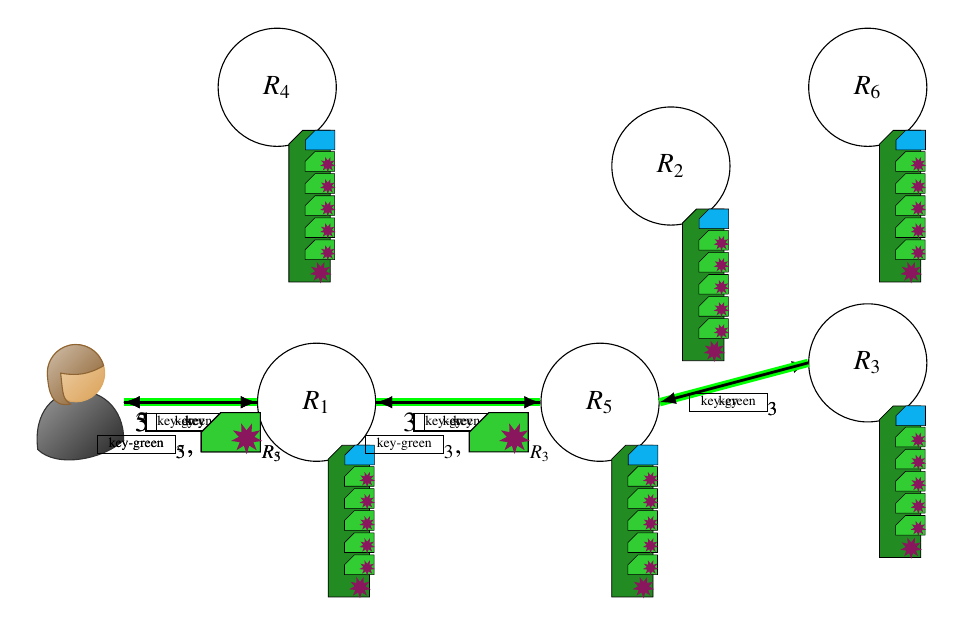
\begin{tikzpicture}
  \node[person,shirt=black,female,minimum size=1.1cm] (user1) at (3,-1) {};


  \begin{pgfonlayer}{background}

    \node[circle,draw,minimum size=1.5cm] (R1) at (6, -1) {$R_1$};
    \node [anchor=north,inner sep=0pt] (cons) at ($(R1.south east)+(-.15, 0)$)
     {\scalebox{.7} { \docendive} };
    \node [anchor=north,inner sep=0pt] (netdoc) at ($(cons.north east)+(-.15, 0)$)
    {\scalebox{0.5}{\netdocunsigned }};
    \node [anchor=north,inner sep=0pt] (d1) at ($(netdoc.south)+(0,0)$)
    {\scalebox{0.5}{\snipdoc}};
    \node [anchor=north,inner sep=0pt] (d2) at (d1.south)
    {\scalebox{0.5}{\snipdoc}};
    \node [anchor=north,inner sep=0pt] (d3) at (d2.south)
    {\scalebox{0.5}{\snipdoc}};
    \node [anchor=north,inner sep=0pt] (d4) at (d3.south)
    {\scalebox{0.5}{\snipdoc}};
    \node [anchor=north,inner sep=0pt] (d5) at (d4.south)
    {\scalebox{0.5}{\snipdoc}};

    \node[circle,draw,minimum size=1.5cm] (R2) at (10.5, 2) {$R_2$};
    \node [anchor=north,inner sep=0pt] (cons) at ($(R2.south east)+(-.15, 0)$)
     {\scalebox{.7} { \docendive} };
    \node [anchor=north,inner sep=0pt] (netdoc) at ($(cons.north east)+(-.15, 0)$)
    {\scalebox{0.5}{\netdocunsigned }};
    \node [anchor=north,inner sep=0pt] (d1) at ($(netdoc.south)+(0,0)$)
    {\scalebox{0.5}{\snipdoc}};
    \node [anchor=north,inner sep=0pt] (d2) at (d1.south)
    {\scalebox{0.5}{\snipdoc}};
    \node [anchor=north,inner sep=0pt] (d3) at (d2.south)
    {\scalebox{0.5}{\snipdoc}};
    \node [anchor=north,inner sep=0pt] (d4) at (d3.south)
    {\scalebox{0.5}{\snipdoc}};
    \node [anchor=north,inner sep=0pt] (d5) at (d4.south)
    {\scalebox{0.5}{\snipdoc}};

    \node[circle,draw,minimum size=1.5cm] (R3) at (13, -.5) {$R_3$};
    \node [anchor=north,inner sep=0pt] (cons) at ($(R3.south east)+(-.15, 0)$)
     {\scalebox{.7} { \docendive} };
    \node [anchor=north,inner sep=0pt] (netdoc) at ($(cons.north east)+(-.15, 0)$)
    {\scalebox{0.5}{\netdocunsigned }};
    \node [anchor=north,inner sep=0pt] (d1) at ($(netdoc.south)+(0,0)$)
    {\scalebox{0.5}{\snipdoc}};
    \node [anchor=north,inner sep=0pt] (d2) at (d1.south)
    {\scalebox{0.5}{\snipdoc}};
    \node [anchor=north,inner sep=0pt] (d3) at (d2.south)
    {\scalebox{0.5}{\snipdoc}};
    \node [anchor=north,inner sep=0pt] (d4) at (d3.south)
    {\scalebox{0.5}{\snipdoc}};
    \node [anchor=north,inner sep=0pt] (d5) at (d4.south)
    {\scalebox{0.5}{\snipdoc}};


    \node[circle,draw,minimum size=1.5cm] (R4) at (5.5, 3) {$R_4$};
    \node [anchor=north,inner sep=0pt] (cons) at ($(R4.south east)+(-.15, 0)$)
     {\scalebox{.7} { \docendive} };
    \node [anchor=north,inner sep=0pt] (netdoc) at ($(cons.north east)+(-.15, 0)$)
    {\scalebox{0.5}{\netdocunsigned }};
    \node [anchor=north,inner sep=0pt] (d1) at ($(netdoc.south)+(0,0)$)
    {\scalebox{0.5}{\snipdoc}};
    \node [anchor=north,inner sep=0pt] (d2) at (d1.south)
    {\scalebox{0.5}{\snipdoc}};
    \node [anchor=north,inner sep=0pt] (d3) at (d2.south)
    {\scalebox{0.5}{\snipdoc}};
    \node [anchor=north,inner sep=0pt] (d4) at (d3.south)
    {\scalebox{0.5}{\snipdoc}};
    \node [anchor=north,inner sep=0pt] (d5) at (d4.south)
    {\scalebox{0.5}{\snipdoc}};

    \node[circle,draw,minimum size=1.5cm] (R5) at (9.6, -1) {$R_5$};
    \node [anchor=north,inner sep=0pt] (cons) at ($(R5.south east)+(-.15, 0)$)
     {\scalebox{.7} { \docendive} };
    \node [anchor=north,inner sep=0pt] (netdoc) at ($(cons.north east)+(-.15, 0)$)
    {\scalebox{0.5}{\netdocunsigned }};
    \node [anchor=north,inner sep=0pt] (d1) at ($(netdoc.south)+(0,0)$)
    {\scalebox{0.5}{\snipdoc}};
    \node [anchor=north,inner sep=0pt] (d2) at (d1.south)
    {\scalebox{0.5}{\snipdoc}};
    \node [anchor=north,inner sep=0pt] (d3) at (d2.south)
    {\scalebox{0.5}{\snipdoc}};
    \node [anchor=north,inner sep=0pt] (d4) at (d3.south)
    {\scalebox{0.5}{\snipdoc}};
    \node [anchor=north,inner sep=0pt] (d5) at (d4.south)
    {\scalebox{0.5}{\snipdoc}};

    \node[circle,draw,minimum size=1.5cm] (R6) at (13, 3) {$R_6$};
    \node [anchor=north,inner sep=0pt] (cons) at ($(R6.south east)+(-.15, 0)$)
     {\scalebox{.7} { \docendive} };
    \node [anchor=north,inner sep=0pt] (netdoc) at ($(cons.north east)+(-.15, 0)$)
    {\scalebox{0.5}{\netdocunsigned }};
    \node [anchor=north,inner sep=0pt] (d1) at ($(netdoc.south)+(0,0)$)
    {\scalebox{0.5}{\snipdoc}};
    \node [anchor=north,inner sep=0pt] (d2) at (d1.south)
    {\scalebox{0.5}{\snipdoc}};
    \node [anchor=north,inner sep=0pt] (d3) at (d2.south)
    {\scalebox{0.5}{\snipdoc}};
    \node [anchor=north,inner sep=0pt] (d4) at (d3.south)
    {\scalebox{0.5}{\snipdoc}};
    \node [anchor=north,inner sep=0pt] (d5) at (d4.south)
    {\scalebox{0.5}{\snipdoc}};
  \end{pgfonlayer}

    \draw<1>[line width=1pt,->] (user1.east) -- (R1.west) node [below, midway]
    {$\pgfuseimage{clikey}_1$};

    \draw<2->[draw=green, line width=3pt,-] (user1.east) -- (R1.west) node
    [below, midway] {};
    \draw<2>[line width=1pt,->] (R1.west) -- (user1.east) node [below, midway]
    {$\pgfuseimage{srvkey}_1$};

    \draw<3>[line width=1pt,->] (user1.east) -- (R1.west) node [below, midway]
    {5 $\pgfuseimage{clikey}_5$};

    \draw<4>[line width=1pt,->] (R1.east) -- (R5.west) node [below, midway]
    {$\pgfuseimage{clikey}_5$};


    \draw<5->[draw=green, line width=3pt,-] (R1.east) -- (R5.west) node {};
    \draw<5>[line width=1pt,->] (R5.west) -- (R1.east) node [below, midway]
    {$\pgfuseimage{srvkey}_5$};

    \draw<6>[line width=1pt,->] (R1.west) -- (user1.east) node [below, midway]
    {$\pgfuseimage{srvkey}_5$, $\snipdoc_{R_5}$};

    \draw<7>[line width=1pt,->] (user1.east) -- (R1.west) node [below, midway]
    {3 $\pgfuseimage{clikey}_3$};

    \draw<8>[line width=1pt,->] (R1.east) -- (R5.west) node [below, midway]
    {3 $\pgfuseimage{clikey}_3$};

    \draw<9>[line width=1pt,->] (R5.east) -- (R3.west) node [below, midway]
    {$\pgfuseimage{clikey}_3$};

    \draw<10->[draw=green, line width=3pt,-] (R5.east) -- (R3.west) node {};
    \draw<10>[line width=1pt,->] (R3.west) -- (R5.east) node [below, midway]
    {$\pgfuseimage{srvkey}_3$};

    \draw<11>[line width=1pt,->] (R5.west) -- (R1.east) node [below, midway]
    {$\pgfuseimage{srvkey}_3$, $\snipdoc_{R_3}$};

    \draw<12>[line width=1pt,->] (R1.west) -- (user1.east) node [below, midway]
    {$\pgfuseimage{srvkey}_3$, $\snipdoc_{R_3}$};

\end{tikzpicture}
\end{frame}

\begin{frame}{What improvements does Walking Onions make?}
  \begin{itemize}
    \item<1-> How to represent relay information to enable oblivious
      selection and individual verification?
    \item<1->[]~
    \item<1-> How to build paths using oblivious relay selection?
    \item<1->[]~
    \item<1-> \textbf{How to perform more efficient circuit construction?}
  \end{itemize}
\end{frame}

\begin{frame}
\frametitle{Single-Pass Walking Onions}
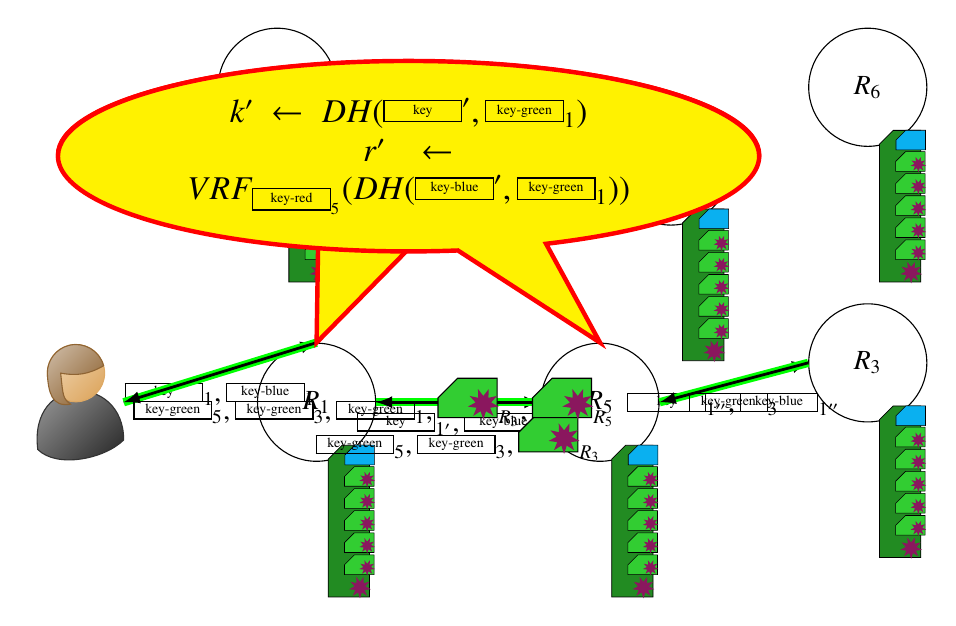
\begin{tikzpicture}
  \node[person,shirt=black,female,minimum size=1.1cm] (user1) at (3,-1) {};

  \begin{pgfonlayer}{background}

    \node[circle,draw,minimum size=1.5cm] (R1) at (6, -1) {$R_1$};
    \node [anchor=north,inner sep=0pt] (cons) at ($(R1.south east)+(-.15, 0)$)
     {\scalebox{.7} { \docendive} };
    \node [anchor=north,inner sep=0pt] (netdoc) at ($(cons.north east)+(-.15, 0)$)
    {\scalebox{0.5}{\netdocunsigned }};
    \node [anchor=north,inner sep=0pt] (d1) at ($(netdoc.south)+(0,0)$)
    {\scalebox{0.5}{\snipdoc}};
    \node [anchor=north,inner sep=0pt] (d2) at (d1.south)
    {\scalebox{0.5}{\snipdoc}};
    \node [anchor=north,inner sep=0pt] (d3) at (d2.south)
    {\scalebox{0.5}{\snipdoc}};
    \node [anchor=north,inner sep=0pt] (d4) at (d3.south)
    {\scalebox{0.5}{\snipdoc}};
    \node [anchor=north,inner sep=0pt] (d5) at (d4.south)
    {\scalebox{0.5}{\snipdoc}};

    \node[circle,draw,minimum size=1.5cm] (R2) at (10.5, 2) {$R_2$};
    \node [anchor=north,inner sep=0pt] (cons) at ($(R2.south east)+(-.15, 0)$)
     {\scalebox{.7} { \docendive} };
    \node [anchor=north,inner sep=0pt] (netdoc) at ($(cons.north east)+(-.15, 0)$)
    {\scalebox{0.5}{\netdocunsigned }};
    \node [anchor=north,inner sep=0pt] (d1) at ($(netdoc.south)+(0,0)$)
    {\scalebox{0.5}{\snipdoc}};
    \node [anchor=north,inner sep=0pt] (d2) at (d1.south)
    {\scalebox{0.5}{\snipdoc}};
    \node [anchor=north,inner sep=0pt] (d3) at (d2.south)
    {\scalebox{0.5}{\snipdoc}};
    \node [anchor=north,inner sep=0pt] (d4) at (d3.south)
    {\scalebox{0.5}{\snipdoc}};
    \node [anchor=north,inner sep=0pt] (d5) at (d4.south)
    {\scalebox{0.5}{\snipdoc}};

    \node[circle,draw,minimum size=1.5cm] (R3) at (13, -.5) {$R_3$};
    \node [anchor=north,inner sep=0pt] (cons) at ($(R3.south east)+(-.15, 0)$)
     {\scalebox{.7} { \docendive} };
    \node [anchor=north,inner sep=0pt] (netdoc) at ($(cons.north east)+(-.15, 0)$)
    {\scalebox{0.5}{\netdocunsigned }};
    \node [anchor=north,inner sep=0pt] (d1) at ($(netdoc.south)+(0,0)$)
    {\scalebox{0.5}{\snipdoc}};
    \node [anchor=north,inner sep=0pt] (d2) at (d1.south)
    {\scalebox{0.5}{\snipdoc}};
    \node [anchor=north,inner sep=0pt] (d3) at (d2.south)
    {\scalebox{0.5}{\snipdoc}};
    \node [anchor=north,inner sep=0pt] (d4) at (d3.south)
    {\scalebox{0.5}{\snipdoc}};
    \node [anchor=north,inner sep=0pt] (d5) at (d4.south)
    {\scalebox{0.5}{\snipdoc}};


    \node[circle,draw,minimum size=1.5cm] (R4) at (5.5, 3) {$R_4$};
    \node [anchor=north,inner sep=0pt] (cons) at ($(R4.south east)+(-.15, 0)$)
     {\scalebox{.7} { \docendive} };
    \node [anchor=north,inner sep=0pt] (netdoc) at ($(cons.north east)+(-.15, 0)$)
    {\scalebox{0.5}{\netdocunsigned }};
    \node [anchor=north,inner sep=0pt] (d1) at ($(netdoc.south)+(0,0)$)
    {\scalebox{0.5}{\snipdoc}};
    \node [anchor=north,inner sep=0pt] (d2) at (d1.south)
    {\scalebox{0.5}{\snipdoc}};
    \node [anchor=north,inner sep=0pt] (d3) at (d2.south)
    {\scalebox{0.5}{\snipdoc}};
    \node [anchor=north,inner sep=0pt] (d4) at (d3.south)
    {\scalebox{0.5}{\snipdoc}};
    \node [anchor=north,inner sep=0pt] (d5) at (d4.south)
    {\scalebox{0.5}{\snipdoc}};

    \node[circle,draw,minimum size=1.5cm] (R5) at (9.6, -1) {$R_5$};
    \node [anchor=north,inner sep=0pt] (cons) at ($(R5.south east)+(-.15, 0)$)
     {\scalebox{.7} { \docendive} };
    \node [anchor=north,inner sep=0pt] (netdoc) at ($(cons.north east)+(-.15, 0)$)
    {\scalebox{0.5}{\netdocunsigned }};
    \node [anchor=north,inner sep=0pt] (d1) at ($(netdoc.south)+(0,0)$)
    {\scalebox{0.5}{\snipdoc}};
    \node [anchor=north,inner sep=0pt] (d2) at (d1.south)
    {\scalebox{0.5}{\snipdoc}};
    \node [anchor=north,inner sep=0pt] (d3) at (d2.south)
    {\scalebox{0.5}{\snipdoc}};
    \node [anchor=north,inner sep=0pt] (d4) at (d3.south)
    {\scalebox{0.5}{\snipdoc}};
    \node [anchor=north,inner sep=0pt] (d5) at (d4.south)
    {\scalebox{0.5}{\snipdoc}};

    \node[circle,draw,minimum size=1.5cm] (R6) at (13, 3) {$R_6$};
    \node [anchor=north,inner sep=0pt] (cons) at ($(R6.south east)+(-.15, 0)$)
     {\scalebox{.7} { \docendive} };
    \node [anchor=north,inner sep=0pt] (netdoc) at ($(cons.north east)+(-.15, 0)$)
    {\scalebox{0.5}{\netdocunsigned }};
    \node [anchor=north,inner sep=0pt] (d1) at ($(netdoc.south)+(0,0)$)
    {\scalebox{0.5}{\snipdoc}};
    \node [anchor=north,inner sep=0pt] (d2) at (d1.south)
    {\scalebox{0.5}{\snipdoc}};
    \node [anchor=north,inner sep=0pt] (d3) at (d2.south)
    {\scalebox{0.5}{\snipdoc}};
    \node [anchor=north,inner sep=0pt] (d4) at (d3.south)
    {\scalebox{0.5}{\snipdoc}};
    \node [anchor=north,inner sep=0pt] (d5) at (d4.south)
    {\scalebox{0.5}{\snipdoc}};


    %%%%%%%%%%%%%%%%%%%%%%%%%%%%%%%%%%%%%%%%%%%%%%%%%%%%%%%%%%%

    \draw<1>[line width=1pt,->] (user1.east) -- (R1.north) node [below, midway]
    {$\pgfuseimage{clikey}_1, \pgfuseimage{clivrfkey}_1$};

    \draw<2>[line width=1pt,->] (R1.east) -- (R5.west) node [below, midway]
    {$\pgfuseimage{clikey}_{1'}, \pgfuseimage{clivrfkey}_{1'}$};

    \draw<3>[line width=1pt,->] (R5.east) -- (R3.west) node [below, midway]
    {$\pgfuseimage{clikey}_{1''}, \pgfuseimage{clivrfkey}_{1''}$};

    \draw<4->[draw=green, line width=3pt,-] (R5.east) -- (R3.west) node {};
    \draw<4>[line width=1pt,->] (R3.west) -- (R5.east) node [below, midway]
    {$\pgfuseimage{srvkey}_3$};

    \draw<5->[draw=green, line width=3pt,-] (R1.east) -- (R5.west) node {};
    \draw<5>[line width=1pt,->] (R5.west) -- (R1.east) node [below, midway]
    {$\pgfuseimage{srvkey}_5, \pgfuseimage{srvkey}_3, \snipdoc_{R_3}$};

    \draw<6->[draw=green, line width=3pt,-] (user1.east) -- (R1.north) node
    [below, midway] {};
    \draw<6>[line width=1pt,->] (R1.north) -- (user1.east) node [above, right]
    {$\pgfuseimage{srvkey}_5, \pgfuseimage{srvkey}_3, \pgfuseimage{srvkey}_1,
    \snipdoc_{R_3}, \snipdoc_{R_5}$};
  \end{pgfonlayer}

  \begin{pgfonlayer}{background}
    \node<2> [fill=yellow,draw=red,ultra thick,font=\large, text
    width=.5\textwidth,anchor=north west,ellipse callout,text centered,callout
    absolute pointer = {($(R1.north)+(0,0)$)}] at (4,3) {$k \leftarrow
    DH(\pgfuseimage{clikey},\pgfuseimage{srvkey}_1)$\\ $r \leftarrow
    VRF_{\pgfuseimage{srvvrfkey}_1}(DH(\pgfuseimage{clivrfkey},\pgfuseimage{srvkey}_1))$
    };

    \node<3> [fill=yellow,draw=red,ultra thick,font=\large, text
    width=.5\textwidth,anchor=north west,ellipse callout,text centered,callout
    absolute pointer = {($(R5.north)+(0,0)$)}] at (4,3) {$k' \leftarrow
    DH(\pgfuseimage{clikey}',\pgfuseimage{srvkey}_1)$\\ $r' \leftarrow
    VRF_{\pgfuseimage{srvvrfkey}_5}(DH(\pgfuseimage{clivrfkey}',\pgfuseimage{srvkey}_1))$ };
  \end{pgfonlayer}

\end{tikzpicture}
\end{frame}


\begin{frame}
  \centering
  \huge
  Performance Evaluation
\end{frame}

\begin{frame}
\frametitle{Bandwidth Results for Tor Relays}
\begin{center}
  \hspace{-1.7cm}
  \begin{minipage}[t] {0.45\linewidth}
    \vspace*{8em}
    \begin{tikzpicture}
        \scalebox{0.62} {
          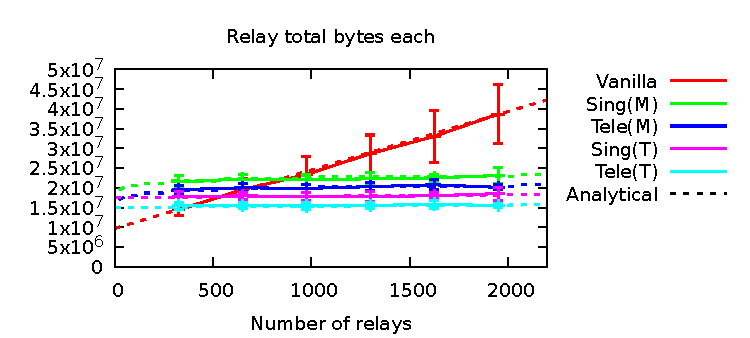
\includegraphics{relay_ss.pdf}
        }
    \end{tikzpicture}
  \end{minipage}
  \hspace{0.6cm}
  \begin{minipage}[t] {0.45\linewidth}
    \vspace*{8em}
    \begin{tikzpicture}
    \scalebox{0.62} {
      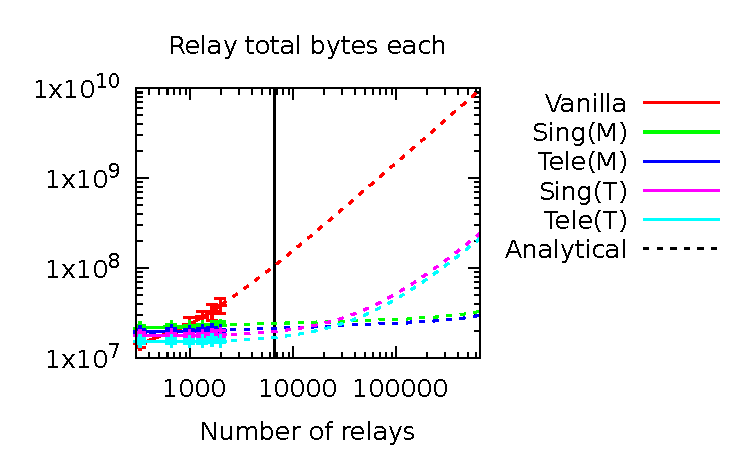
\includegraphics{relay_ss_wide.pdf}
    }
    \end{tikzpicture}
  \end{minipage}
\end{center}
\end{frame}

\begin{frame}
\frametitle{Bandwidth Results for Tor Clients}
\begin{center}
  \hspace{-1.7cm}
  \begin{minipage}[t] {0.45\linewidth}
    \vspace*{8em}
    \begin{tikzpicture}
    \scalebox{0.62} {
      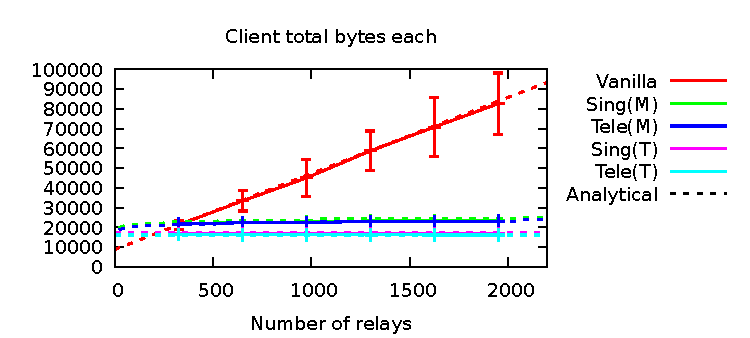
\includegraphics{client_ss.pdf}
    }
    \end{tikzpicture}
  \end{minipage}
  \hspace{0.5cm}
  \begin{minipage}[t] {0.45\linewidth}
    \vspace*{8em}
    \begin{tikzpicture}
    \scalebox{0.62} {
      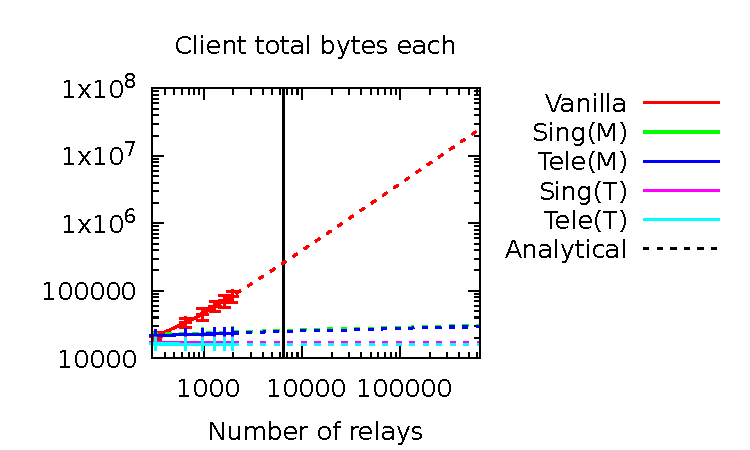
\includegraphics{client_ss_wide.pdf}
    }
    \end{tikzpicture}
  \end{minipage}
\end{center}
\end{frame}

\begin{frame}
\frametitle{Takeaways}
  \begin{itemize}
    \item<1-> The design of Tor today imposes impractical overheads to clients as
      the network scales.
    \item<2-> Walking Onions:
      \begin{itemize}
        \item<3-> Removes the per-relay bandwidth and storage cost to clients, and
        \item<4-> Offers the same security protections against epistemic
      and route capture attacks as prior designs that required a globally
      consistent view.
      \end{itemize}
    \item<5-> Tor has already begun the specification work to integrate
      Walking Onions into the Tor protocol.`
    \item[]~
  \end{itemize}
      \footnotesize{Find our full paper and artifact at

      https://crysp.uwaterloo.ca/software/walkingonions}
\end{frame}

\end{document}

\begin{frame}
\frametitle{}

\begin{table}[t]
\renewcommand{\arraystretch}{1.2}
\caption{Bonus Slide: Comparison of Telescoping, Single-Pass, Current Tor }

\centering
\footnotesize

\CIRCLE=achieved; \Circle=not achieved;
  \LEFTcircle=partially achieved

$\Diamond$=performance property;
  $\dagger$=security property

    \begin{tabular}{|c|c|c|c|c|}
  \hline
  & & Telescop. & Single-Pass & Current Tor \\
  \hline
  $\Diamond$ & Constant-size client download & \CIRCLE & \CIRCLE & \Circle \\
  \hline
  $\Diamond$ & One round trip per circuit built & \Circle & \CIRCLE & \Circle \\
  % Start security properties
  \hline
  $\dagger$ & \raggedright Complete client control of relays selected & \LEFTcircle & \Circle & \CIRCLE \\
  \hline
  $\dagger$ & Forward-secret relay selection& \CIRCLE & \LEFTcircle & \CIRCLE \\
  \hline
  $\dagger$ & Forward secrecy for data & \CIRCLE & \CIRCLE & \CIRCLE \\
  \hline
  $\dagger$ & \raggedright Relays unaware of their positions in paths & \LEFTcircle & \Circle & \LEFTcircle \\
  \hline
\end{tabular}

\end{table}
\end{frame}

\begin{frame}
\frametitle{Complex Path Requirements: Multiple Index Ranges}
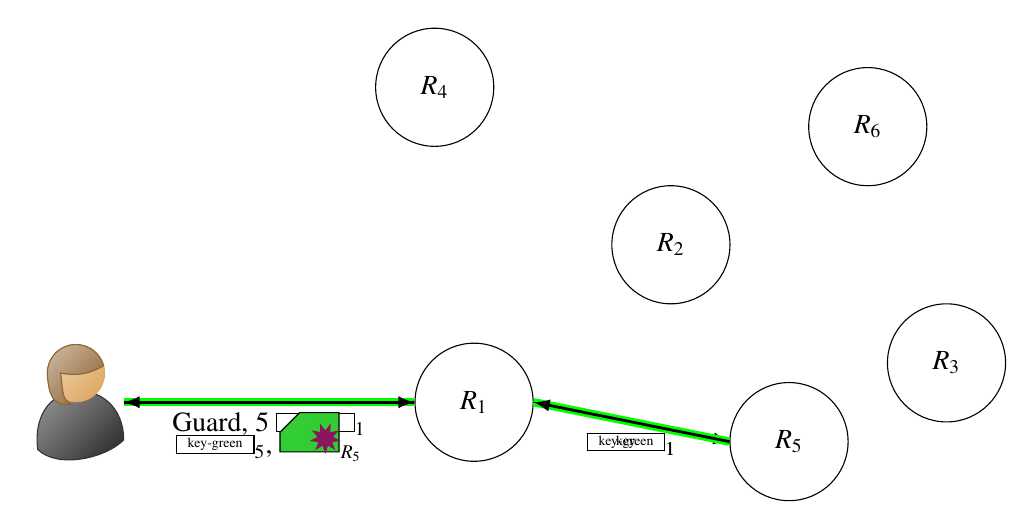
\begin{tikzpicture}
  \node[person,shirt=black,female,minimum size=1.1cm] (user1) at (3,-1) {};

  \begin{pgfonlayer}{background}
    \node[circle,draw,minimum size=1.5cm] (R1) at (8, -1) {$R_1$};
    \node[circle,draw,minimum size=1.5cm] (R2) at (10.5, 1) {$R_2$};
    \node[circle,draw,minimum size=1.5cm] (R3) at (14, -.5) {$R_3$};
    \node[circle,draw,minimum size=1.5cm] (R4) at (7.5, 3) {$R_4$};
    \node[circle,draw,minimum size=1.5cm] (R5) at (12, -1.5) {$R_5$};
    \node[circle,draw,minimum size=1.5cm] (R6) at (13, 2.5) {$R_6$};
  \end{pgfonlayer}
    \draw[draw=green, line width=3pt,-] (user1.east) -- (R1.west) node
    [below, midway] {};
    \draw<1>[line width=1pt,->] (user1.east) -- (R1.west) node [below, midway]
    {Guard, 5 $\pgfuseimage{clikey}_1$};
    \draw<2>[line width=1pt,->] (R1.east) -- (R5.west) node [below, midway]
    {$\pgfuseimage{clikey}_1$};
    \draw<3->[draw=green, line width=3pt,-] (R1.east) -- (R5.west) node {};
    \draw<3>[line width=1pt,->] (R5.west) -- (R1.east) node [below, midway]
    {$\pgfuseimage{srvkey}_1$};
    \draw<4>[line width=1pt,->] (R1.west) -- (user1.east) node [below, midway]
    {$\pgfuseimage{srvkey}_5$, $\snipdoc_{R_5}$};
\end{tikzpicture}
\end{frame}

\begin{frame}
\frametitle{Complex Path Requirements: Delegated Verfiable Selection}
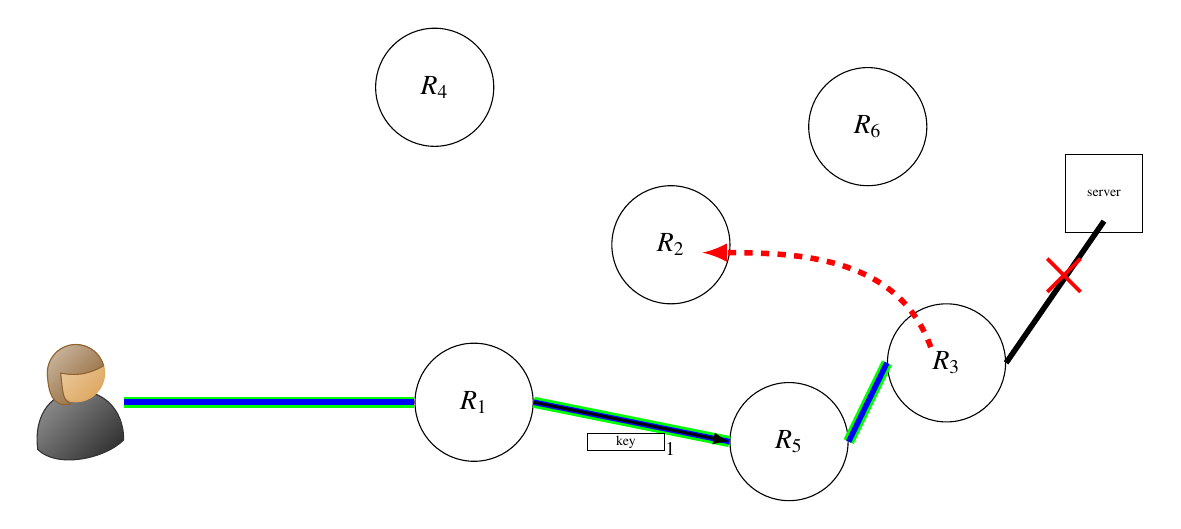
\begin{tikzpicture}
  \node[person,shirt=black,female,minimum size=1.1cm] (user1) at (3,-1) {};

  \begin{pgfonlayer}{background}
    \node (s2) at (16,1.65) {\pgfuseimage{server}};
    \node[circle,draw,minimum size=1.5cm] (R1) at (8, -1) {$R_1$};
    \node[circle,draw,minimum size=1.5cm] (R2) at (10.5, 1) {$R_2$};
    \node[circle,draw,minimum size=1.5cm] (R3) at (14, -.5) {$R_3$};
    \node[circle,draw,minimum size=1.5cm] (R4) at (7.5, 3) {$R_4$};
    \node[circle,draw,minimum size=1.5cm] (R5) at (12, -1.5) {$R_5$};
    \node[circle,draw,minimum size=1.5cm] (R6) at (13, 2.5) {$R_6$};
  \end{pgfonlayer}
    \draw[draw=green, line width=4pt,-] (user1.east) -- (R1.west) node
    [below, midway] {};
    \draw[draw=green, line width=4pt,-] (R1.east) -- (R5.west) node {};
    \draw[draw=green, line width=4pt,-] (R5.east) -- (R3.west) node {};

    \draw[draw=blue, line width=2pt,-] (user1.east) -- (R1.west) node
    [below, midway] {};
    \draw[draw=blue, line width=2pt,-] (R1.east) -- (R5.west) node {};
    \draw[draw=blue, line width=2pt,-] (R5.east) -- (R3.west) node {};
    \draw [line width=2pt,-] (R3.east) to (16, 1.3);
    \node<2> [inner sep=1pt,font=\Huge,text=red] (block) at (15.5, .6) {$\mathbf{\times}$};
    \draw<2> [line width=2pt,draw=red,dashed,->] ($(R3)+(-.2,.2)$) to[out=110,in=0] ($(R2)+(.4,-.1)$);
    \draw<2>[line width=1pt,->] (R1.east) -- (R5.west) node [below, midway]
    {$\pgfuseimage{clikey}_1$};
\end{tikzpicture}
\end{frame}


% Bonus slides
\begin{frame}
\frametitle{Simulation}
TODO Simulation description
\end{frame}

\begin{frame}
\frametitle{CPU}
\end{frame}
